The most recent underwater robot is the Ocean One by Khatib et. al. \cite{oceanone}.
The Ocean One is a high degree of freedom upper body humanoid robot with the lower body of an unmanned underwater vehicle (UUV).
This impressive robot can move around and manipulate objects with its highly sensitive tactile sensors on its manipulators.
The robot has been used to explore ship wrecks of historic interest and help excavate the artifacts.
The Ocean One is designed for its manipulation abilities.
The thrusters that allow the Ocean One to move through the water have the problem of most other UUVs where it stirs up silt and debris which reduces visibility.

\begin{figure*}[th]
\centering
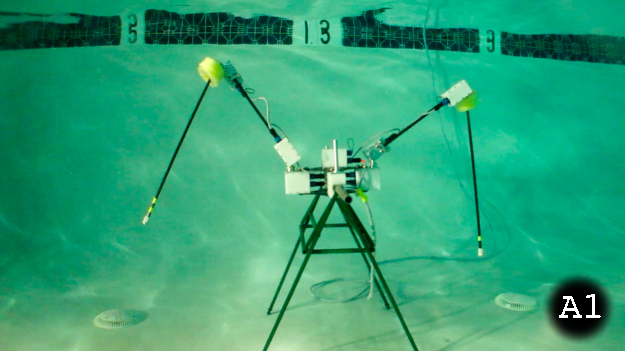
\includegraphics[width=0.66\columnwidth]{./img/a1.pdf}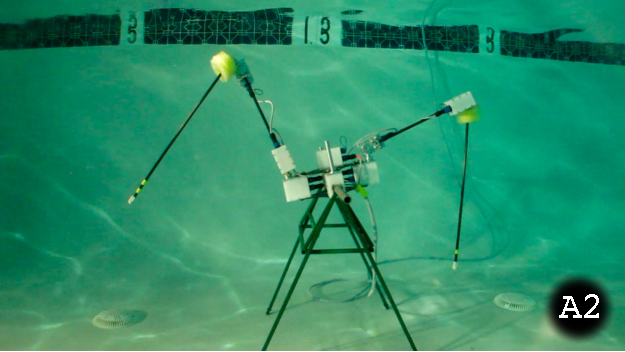
\includegraphics[width=0.66\columnwidth]{./img/a2.pdf}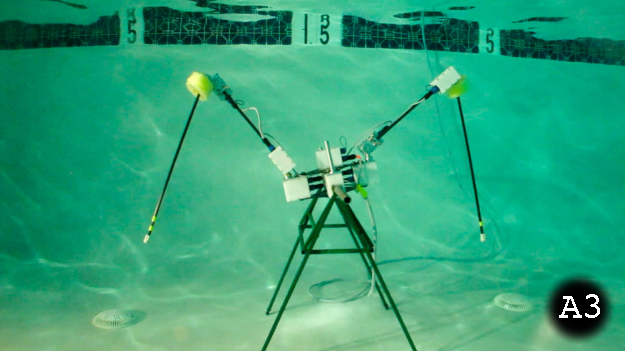
\includegraphics[width=0.66\columnwidth]{./img/a3.pdf}
\caption{AquaShoko underwater robot operating underwater controlling the attitude of its body via our method described in \ref{sec:stable}. The robot is being commanded with step input for the desired body attitude in the $Y-axis$ (out of the page).  (\textbf{A1-A3}) Step input of 0.2 $rad$, initial orientation 0.0 $rad$.  }
\label{fig:underwarter}
\end{figure*}


The Crabster (CR200) by the Korea Research Institute of Ships \& Ocean Engineering (KRISO) developed a legged underwater vehicle that does not need thrusters to move \cite{seacrab}.
It can navigate in upto 200$m$ water with passengers on board.
The legs of the robot were specifically designed to allow it to both swim and walk on the sea floor.
In their work they used the work of Kim et. al. \cite{crab1} and Jun et. al. for the communications and hydrodynamics of the legs respectively. 
These lessons help guide us in the choice of communication methods and size/shape of our legs.

Additionally JY Kim et. al. \cite{crab3} focused on creating a six-legged underwater UUV.
This is important because they also used their front two legs as manipulators.


From this previous work we decided to start by designing a legged robot with long thin legs to reduce the hydrodynamic effects.
Tethered communications and power was chosen for initial testing.
When adding manipulation in future work we will have six legs.  
Our current test platform has four legs because we want to focus on initial platform development before increasing the complexity of the system.

